\documentclass[10pt, a4paper, twocolumn]{article}

% ── Packages ──────────────────────────────────────────────────────────────────
\usepackage[a4paper, top=2.5cm, bottom=2.5cm, left=1.8cm, right=1.8cm, columnsep=0.6cm]{geometry}
\usepackage{xcolor}
\usepackage{titlesec}
\usepackage{graphicx}
\usepackage{booktabs}
\usepackage{array}
\usepackage{multirow}
\usepackage{amsmath}
\usepackage{amssymb}
\usepackage{hyperref}
\usepackage{enumitem}
\usepackage{microtype}
\usepackage{fancyhdr}
\usepackage{tcolorbox}
\usepackage{listings}
\usepackage{caption}
\usepackage{float}
\usepackage{times}
\usepackage{parskip}
\usepackage{tabularx}

\tcbuselibrary{skins, breakable}

% ── Colors ────────────────────────────────────────────────────────────────────
\definecolor{navyblue}{RGB}{26, 50, 89}
\definecolor{lightgray}{RGB}{245, 245, 245}
\definecolor{linkblue}{RGB}{0, 102, 204}

% ── Section Styling (full-width colored box, white text) ──────────────────────


\titleformat{\subsection}
  {\normalfont\normalsize\bfseries}
  {\thesubsection}
  {0.5em}
  {}
\titlespacing*{\subsection}{0pt}{8pt}{3pt}

% ── Hyperlinks ────────────────────────────────────────────────────────────────
\hypersetup{colorlinks=true, linkcolor=linkblue, urlcolor=linkblue, citecolor=linkblue}

% ── Header / Footer ───────────────────────────────────────────────────────────
\pagestyle{fancy}
\fancyhf{}
\rhead{\small EE200}
\lhead{\small Question 1 Report}
\cfoot{\small \thepage}
\renewcommand{\headrulewidth}{0.4pt}

% ── Table & Caption ───────────────────────────────────────────────────────────
\renewcommand{\arraystretch}{1.3}
\captionsetup{font=small, labelfont=bf, skip=4pt}

% ── Code listing ──────────────────────────────────────────────────────────────
\lstset{
  backgroundcolor=\color{lightgray},
  basicstyle=\ttfamily\scriptsize,
  breaklines=true,
  frame=single,
  numbers=left,
  numberstyle=\tiny\color{gray},
  keywordstyle=\color{navyblue}\bfseries,
  commentstyle=\color{gray}\itshape,
}

% ── Closed-border table helper ────────────────────────────────────────────────
% Use \hline at top, \hline between rows, \hline at bottom, with | for vertical lines

% ─────────────────────────────────────────────────────────────────────────────
\begin{document}

% ── Title Page (single column) ────────────────────────────────────────────────
\twocolumn[{
\begin{@twocolumnfalse}
  \begin{center}
    \vspace{2.0cm}
    {\LARGE \textbf{EE200: Signals, Systems and Networks}}\\[4pt]
    {\LARGE \textbf{Course Project}}\\[10pt]
    {\Large \textsc{Question 1 Report}}\\[40pt]







    \Large\textsc{Team Members:}\\[10pt]

    \makebox[0.3\textwidth][l]{\textbf{240622 Manish Kajla}}\\
    \makebox[0.3\textwidth][l]{\textbf{241114 Utkarsh Aman}}\\[90pt]

    

    \Large{\textbf{Abstract}}\\[15pt]
    \begin{minipage}{0.90\textwidth}
      \large\itshape\centering
      

        This report presents the analysis of two image processing problems using concepts from signals and systems. In \textit{Frequency Forensics: The Ghost Signal}, a grayscale image corrupted by periodic interference is transformed into the frequency domain using the two-dimensional Discrete Fourier Transform (DFT). The resulting spectrum is analyzed to identify unwanted frequency components, which are then suppressed using a notch filter. The image is subsequently reconstructed using the inverse DFT to recover the hidden information.
        
        In \textit{Digital Detective: Missing Boundaries}, edge detection is performed using the Sobel operator to identify regions of rapid intensity variation. The influence of noise on edge extraction is examined, and Gaussian smoothing is applied to improve boundary detection. The obtained results demonstrate the effectiveness of frequency-domain filtering for image restoration and gradient-based methods for feature extraction, highlighting important applications of signal processing techniques in image analysis.
        

    \end{minipage}\\[12pt]
   
    \vspace{0.2cm}
  \end{center}
\end{@twocolumnfalse}
}]
\clearpage
\tableofcontents
\clearpage

\section{Introduction}
Digital images can be treated as two-dimensional discrete signals whose intensity values vary along both spatial dimensions. By applying signal processing techniques, images can be analyzed in either the spatial domain or the frequency domain to extract useful information, remove unwanted distortions and identify important features. Such techniques are widely used in communication systems, surveillance, medical imaging and computer vision applications.

The first part of this report, \textit{Frequency Forensics: The Ghost Signal}, investigates the recovery of information hidden beneath periodic interference. The corrupted image is transformed into the frequency domain using the two-dimensional Discrete Fourier Transform (DFT), where the interference appears as distinct spectral components. By identifying and suppressing these components through frequency-domain filtering, the original image can be reconstructed and the hidden information recovered.

The second part, \textit{Digital Detective: Missing Boundaries}, focuses on edge detection using the Sobel operator. Image gradients are used to locate regions of rapid intensity variation that correspond to object boundaries. The effects of noise and the role of Gaussian smoothing in improving edge detection performance are also examined.

Through these experiments, the practical application of Fourier analysis, filtering and gradient-based image processing techniques is demonstrated for image restoration and feature extraction.



% ─────────────────────────────────────────────────────────────────────────────

\section{Theoretical Background}

\subsection{Images as Two-Dimensional Signals}
A grayscale image can be represented as a two-dimensional discrete signal I(x,y), where each pixel location (x,y) corresponds to an intensity value. Similar to one-dimensional signals, images can be analyzed in different domains to reveal information that may not be immediately visible in the spatial representation.


\subsection{Two-Dimensional Discrete Fourier Transform}

The two-dimensional Discrete Fourier Transform (DFT) converts an image from the spatial domain into the frequency domain and is defined as

\begin{equation}
F(u,v)=\sum_{x=0}^{M-1}\sum_{y=0}^{N-1}
I(x,y)e^{-j2\pi\left(\frac{ux}{M}+\frac{vy}{N}\right)}
\end{equation}

where I(x,y) is the image and F(u,v) represents its frequency-domain representation. The corresponding inverse transform is

\begin{equation}
I(x,y)=\frac{1}{MN}
\sum_{u=0}^{M-1}\sum_{v=0}^{N-1}
F(u,v)e^{j2\pi\left(\frac{ux}{M}+\frac{vy}{N}\right)}
\end{equation}

which reconstructs the original image from its frequency components.

\subsection{Periodic Noise in the Frequency Domain}

Periodic interference appears as localized high-energy peaks in the Fourier spectrum. Unlike useful image information, which is generally concentrated around the low-frequency region, periodic noise produces distinct symmetric spikes that can be identified and removed using frequency-domain filtering techniques such as notch filters.

\subsection{Image Gradients and Edge Detection}

Edges correspond to regions where image intensity changes rapidly. These changes can be detected using the image gradient

\begin{equation}
\nabla I=
\begin{bmatrix}
\frac{\partial I}{\partial x}\
\frac{\partial I}{\partial y}
\end{bmatrix}
\end{equation}

The gradient magnitude is given by

\begin{equation}
|\nabla I|=\sqrt{G_x^2+G_y^2}
\end{equation}

where $G_x$ and $G_y$ represent the intensity changes along the horizontal and vertical directions.

\subsection{The Sobel Operator}

The Sobel operator estimates image gradients using convolution with the following kernels:

\begin{equation}
S_x = 
\begin{bmatrix}
-1 & 0 & 1 \\
-2 & 0 & 2 \\
-1 & 0 & 1
\end{bmatrix}
\end{equation}

\begin{equation}
S_y=
\begin{bmatrix}
-1 & -2 & -1\\
0 & 0 & 0\\
1 & 2 & 1
\end{bmatrix}
\end{equation}

These kernels detect horizontal and vertical intensity variations, allowing object boundaries and structural features within the image to be identified.
% ─────────────────────────────────────────────────────────────────────────────

\section{Q1A: Frequency Forensics – The Ghost Signal}

\subsection{Problem Overview}

The provided image (shown in Figure \ref{fig:corrupted_image}) appears heavily corrupted by a repetitive interference pattern that obscures the underlying information. Although the corruption is difficult to analyze directly in the spatial domain, periodic disturbances produce distinct signatures in the frequency domain. The objective of this task is to identify the frequency components responsible for the corruption, suppress them using an appropriate filtering technique, and reconstruct the image to recover the hidden content. This process forms a Frequency-Domain Image Recovery System based on Fourier analysis and filtering.

\begin{figure}[H]
  \centering
  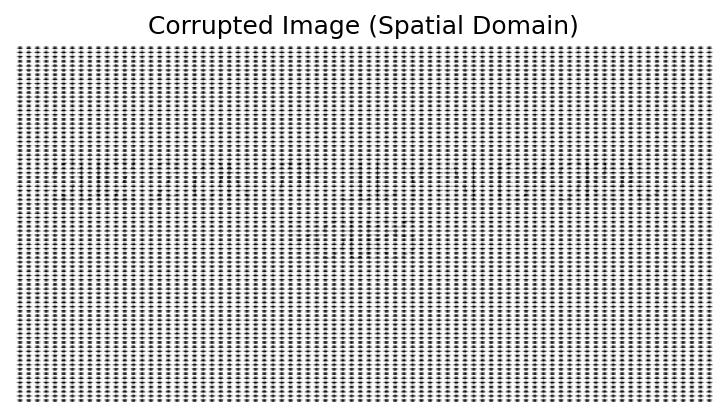
\includegraphics[width=0.85\columnwidth]{plots/corrupted_image.png}
  \caption{Corrupted grayscale image containing periodic interference patterns (spatial domain).}
  \label{fig:corrupted_image}
\end{figure}

\subsection{Methodology}

The recovery process begins by loading the corrupted grayscale image and computing its two-dimensional Discrete Fourier Transform (DFT). The resulting spectrum is shifted using the \texttt{fftshift()} operation so that the low-frequency components are located at the center of the image. The magnitude spectrum is then analyzed in both linear and logarithmic (dB) scales to identify dominant frequency components.

Periodic interference appears as bright symmetric peaks away from the central low-frequency region. These peaks are identified and suppressed using a notch-reject filter. After filtering, the modified spectrum is transformed back to the spatial domain using the inverse DFT, producing a restored image. The corrupted image, frequency spectrum, filtered spectrum and reconstructed image are then compared to evaluate the effectiveness of the restoration process.

\subsection{Frequency Spectrum Analysis}

The Fourier transform decomposes the image into its constituent frequency components. Most of the useful image information is concentrated around the low-frequency region near the center of the shifted spectrum, while fine details and noise occupy higher frequency regions.

The magnitude spectrum was visualized in both linear and dB scales (as shown in Figure \ref{fig:magnitude_spectrum}). While the linear spectrum highlights the strongest frequency components, the dB spectrum provides improved visibility of weaker spectral features by compressing the dynamic range. Examination of the spectrum revealed several isolated bright peaks located symmetrically about the center, indicating the presence of periodic interference within the image.

\begin{figure*}[t]
  \centering
  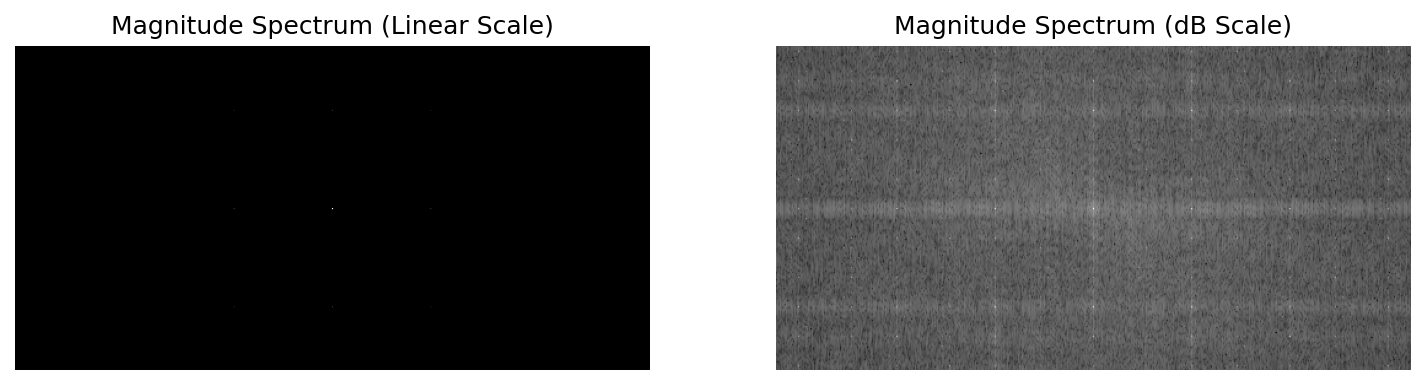
\includegraphics[width=0.85\textwidth]{plots/magnitude_spectrum.png}
  \caption{2D DFT Magnitude Spectrum of the corrupted image. Left: Linear scale, which highlights the DC component. Right: Logarithmic (dB) scale, which compresses the dynamic range to make the symmetric periodic interference spikes clearly visible.}
  \label{fig:magnitude_spectrum}
\end{figure*}

\subsection{Identification of Interference Components}

Periodic noise exhibits a characteristic behavior in the frequency domain by appearing as discrete spectral spikes. These spikes differ from natural image content, which generally forms a continuous distribution concentrated around low frequencies. The observed peaks were located away from the central region and occurred in symmetric pairs, confirming that they originated from periodic interference rather than meaningful image information.

By analyzing the location and intensity of these peaks, the frequency components responsible for the corruption were identified and selected for suppression.

\subsection{Design of the Notch Filter}

To remove the interference, a notch-reject filter was designed in the frequency domain. The filter selectively suppresses frequency components corresponding to the identified spectral peaks while preserving the remaining frequencies.

The filter mask was constructed by placing circular rejection regions around the detected interference frequencies (shown in Figure \ref{fig:notch_mask}). The radius of these regions determines the amount of suppression applied. A small radius may leave residual noise, whereas an excessively large radius can remove useful image information and introduce distortion. Therefore, an appropriate balance was maintained between noise removal and information preservation.

\begin{figure}[H]
  \centering
  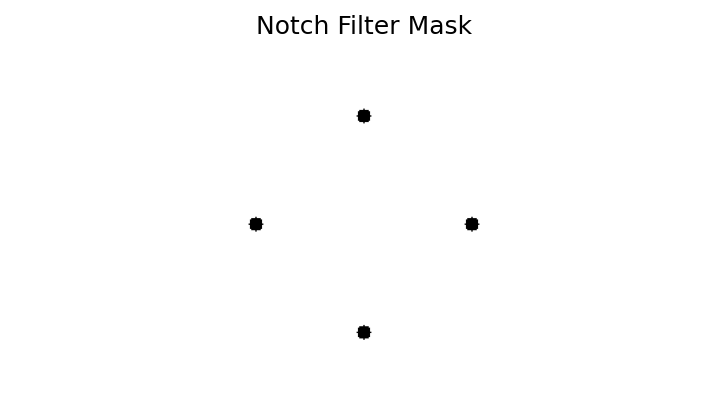
\includegraphics[width=0.85\columnwidth]{plots/notch_mask.png}
  \caption{Custom-designed Notch Filter Mask. The dark circles represent the regions set to zero to suppress the periodic interference spikes, while the bright region represents frequencies that are preserved.}
  \label{fig:notch_mask}
\end{figure}

\subsection{Image Reconstruction and Results}

After applying the notch filter, the modified spectrum was transformed back into the spatial domain using the inverse DFT. The reconstructed image (shown in Figure \ref{fig:recovered_image}) exhibited a significant reduction in periodic interference compared to the original corrupted image. A side-by-side comparison is shown in Figure \ref{fig:q1a_comparison}.

Visual comparison of the corrupted image, magnitude spectrum, filtered spectrum and reconstructed image confirmed that the dominant interference components had been successfully suppressed. The hidden content became considerably more visible after filtering, demonstrating the effectiveness of frequency-domain restoration techniques for periodic noise removal.

\begin{figure}[H]
  \centering
  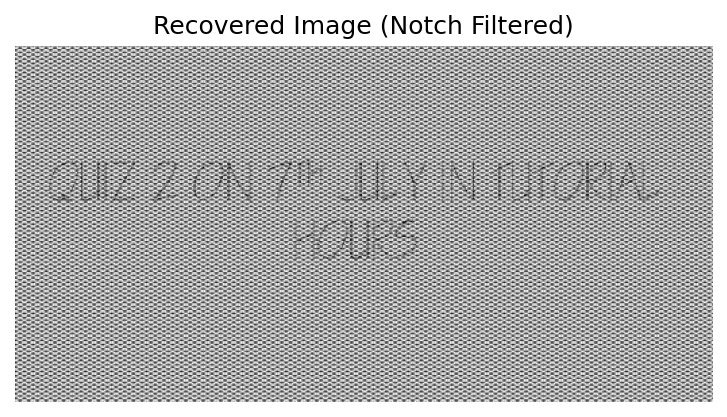
\includegraphics[width=0.85\columnwidth]{plots/recovered_image.png}
  \caption{Reconstructed image (spatial domain) after applying the Notch Filter in the frequency domain, successfully revealing the hidden message.}
  \label{fig:recovered_image}
\end{figure}

\begin{figure*}[t]
  \centering
  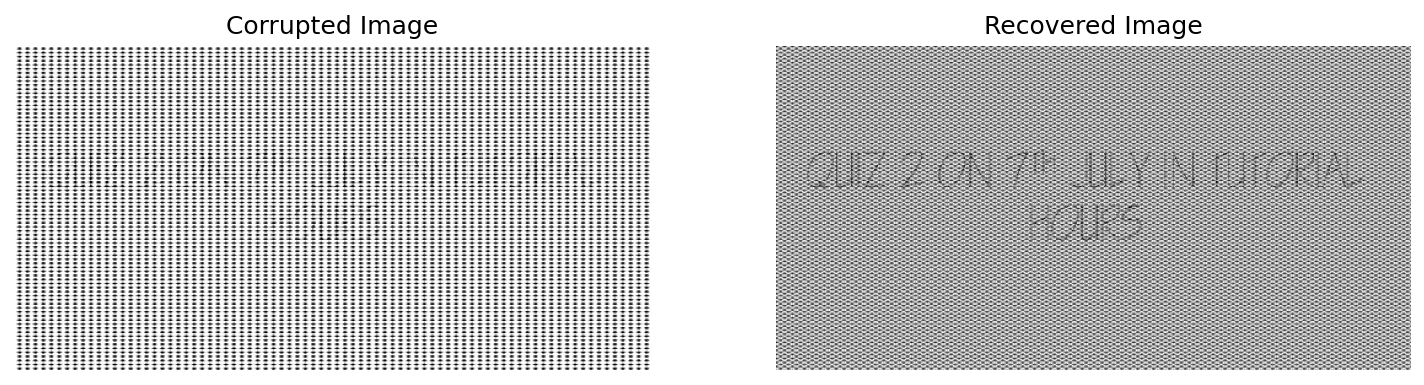
\includegraphics[width=0.85\textwidth]{plots/q1a_comparison.png}
  \caption{Side-by-side comparison between the original corrupted image (left) and the recovered image after frequency-domain notch filtering (right).}
  \label{fig:q1a_comparison}
\end{figure*}

% ─────────────────────────────────────────────────────────────────────────────

\section{Q1B: Digital Detective – Missing Boundaries}

\subsection{Problem Overview}

Edges represent locations of rapid intensity variation and often correspond to object boundaries within an image. Since a significant portion of structural information is contained within edges, accurate edge detection is an important step in many image processing and computer vision applications.

The objective of this task is to use the Sobel operator to detect boundaries within the provided image and analyze the influence of noise and smoothing on edge detection performance.

\subsection{Methodology}

The input image (shown in Figure \ref{fig:missing_boundaries_input}) was first converted into grayscale form and processed using the Sobel operator. Separate convolution operations were performed using horizontal and vertical Sobel kernels to estimate intensity gradients along both spatial directions.

The resulting gradient components were combined to obtain the overall gradient magnitude, which represents the strength of edges present in the image. To investigate the effect of noise, edge detection was performed both before and after Gaussian smoothing, and the resulting edge maps were compared.

\begin{figure}[H]
  \centering
  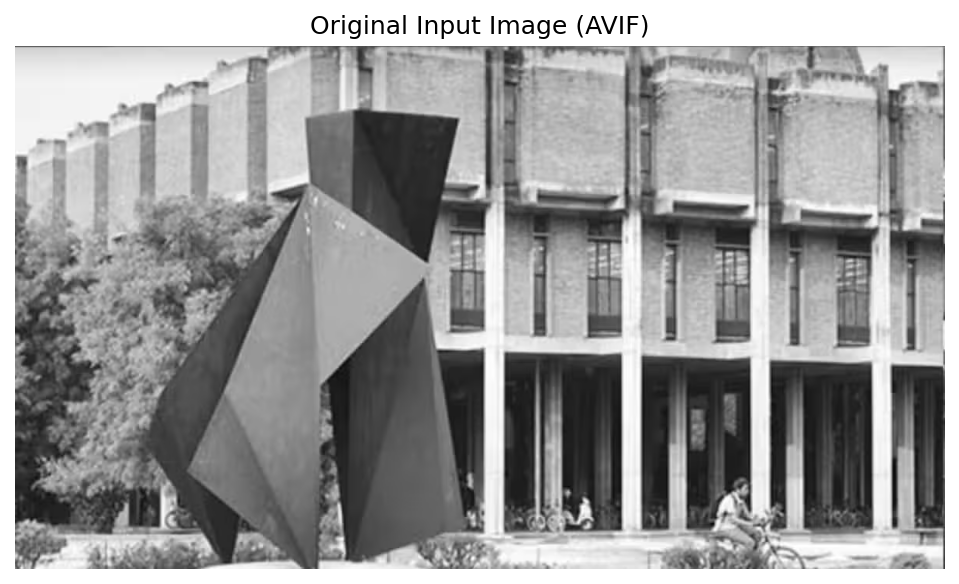
\includegraphics[width=0.85\columnwidth]{plots/missing_boundaries_input.png}
  \caption{Original input image for Q1B (boundary detection).}
  \label{fig:missing_boundaries_input}
\end{figure}

\subsection{Sobel Edge Detection}

The Sobel operator estimates first-order image derivatives and highlights regions of rapid intensity variation. Convolution with the horizontal kernel produces the gradient component ($G_x$), while convolution with the vertical kernel produces ($G_y$).

The final edge magnitude was computed using

\begin{equation}
|\nabla I| = \sqrt{G_x^2 + G_y^2}
\end{equation}

where larger values correspond to stronger edges. The resulting edge map (shown in Figure \ref{fig:sobel_unsmoothed}) successfully highlighted major object boundaries and structural features present in the image, but is heavily corrupted by high-frequency background noise.

\begin{figure*}[t]
  \centering
  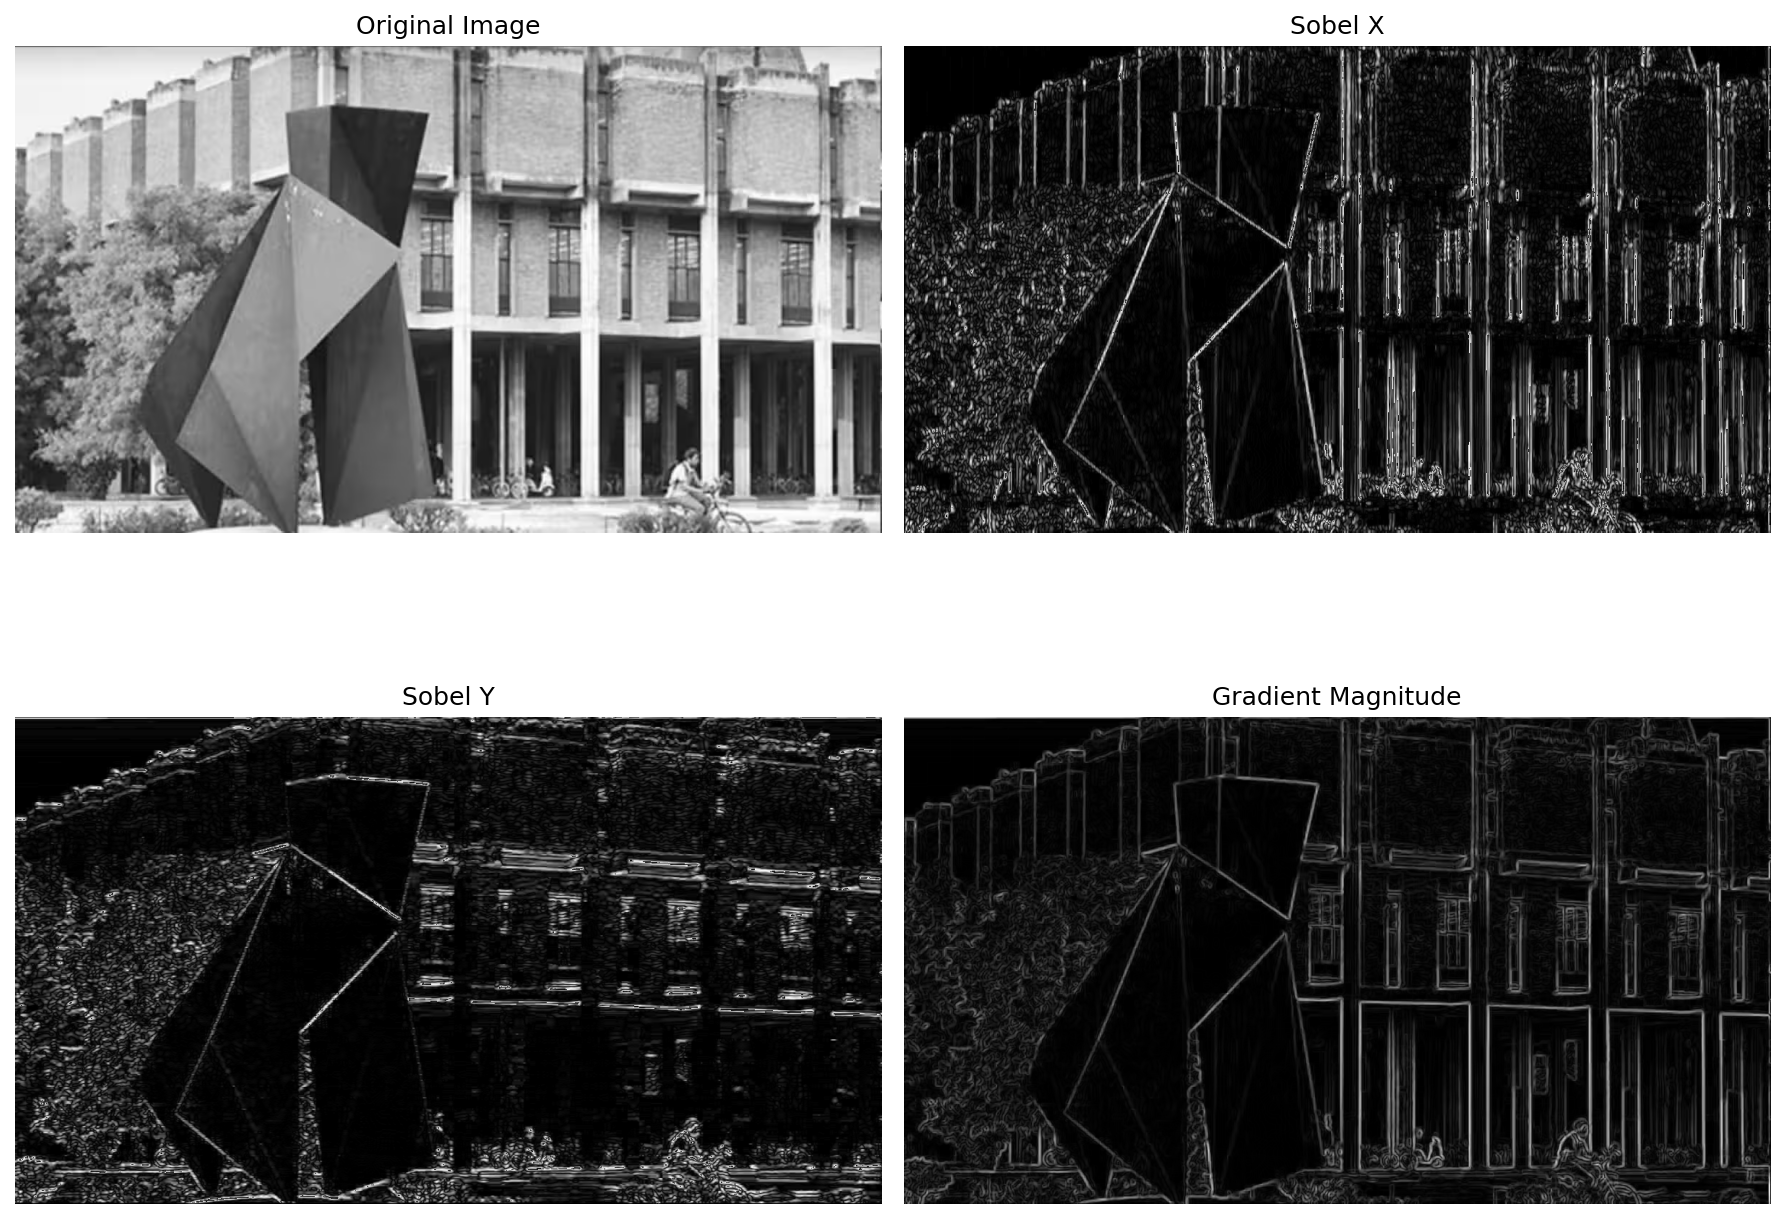
\includegraphics[width=0.85\textwidth]{plots/sobel_unsmoothed.png}
  \caption{Sobel edge detection results on the raw unsmoothed image. From top-left to bottom-right: Original image, horizontal gradient $G_x$, vertical gradient $G_y$, and gradient magnitude. The gradient magnitude is heavily corrupted by high-frequency background noise.}
  \label{fig:sobel_unsmoothed}
\end{figure*}

\subsection{Effect of Noise and Gaussian Smoothing}

Noise introduces random intensity fluctuations that can be incorrectly interpreted as edges by derivative-based operators. As a result, edge maps generated from noisy images often contain false boundaries and fragmented edge structures.

To reduce this effect, Gaussian smoothing was applied prior to edge detection (the smoothed image is shown in Figure \ref{fig:smoothed_image}). The smoothing operation attenuates high-frequency noise while preserving significant image structures. The resulting edge map (shown in Figure \ref{fig:sobel_smoothed}) exhibited improved continuity and reduced false detections, demonstrating the importance of preprocessing before gradient-based edge extraction.

\begin{figure}[H]
  \centering
  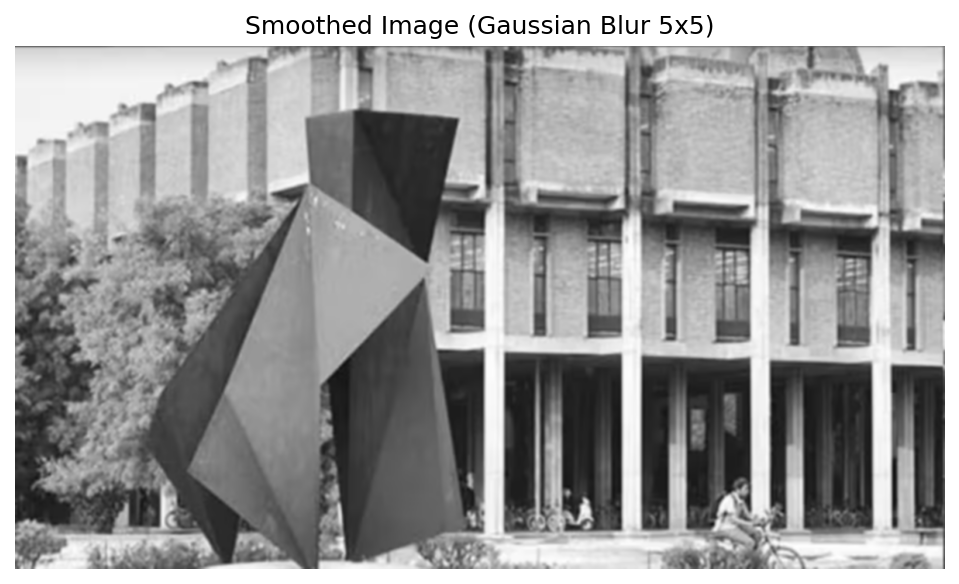
\includegraphics[width=0.85\columnwidth]{plots/smoothed_image.png}
  \caption{Input image after applying a $5\times 5$ Gaussian smoothing filter, which suppresses high-frequency noise.}
  \label{fig:smoothed_image}
\end{figure}

\begin{figure*}[t]
  \centering
  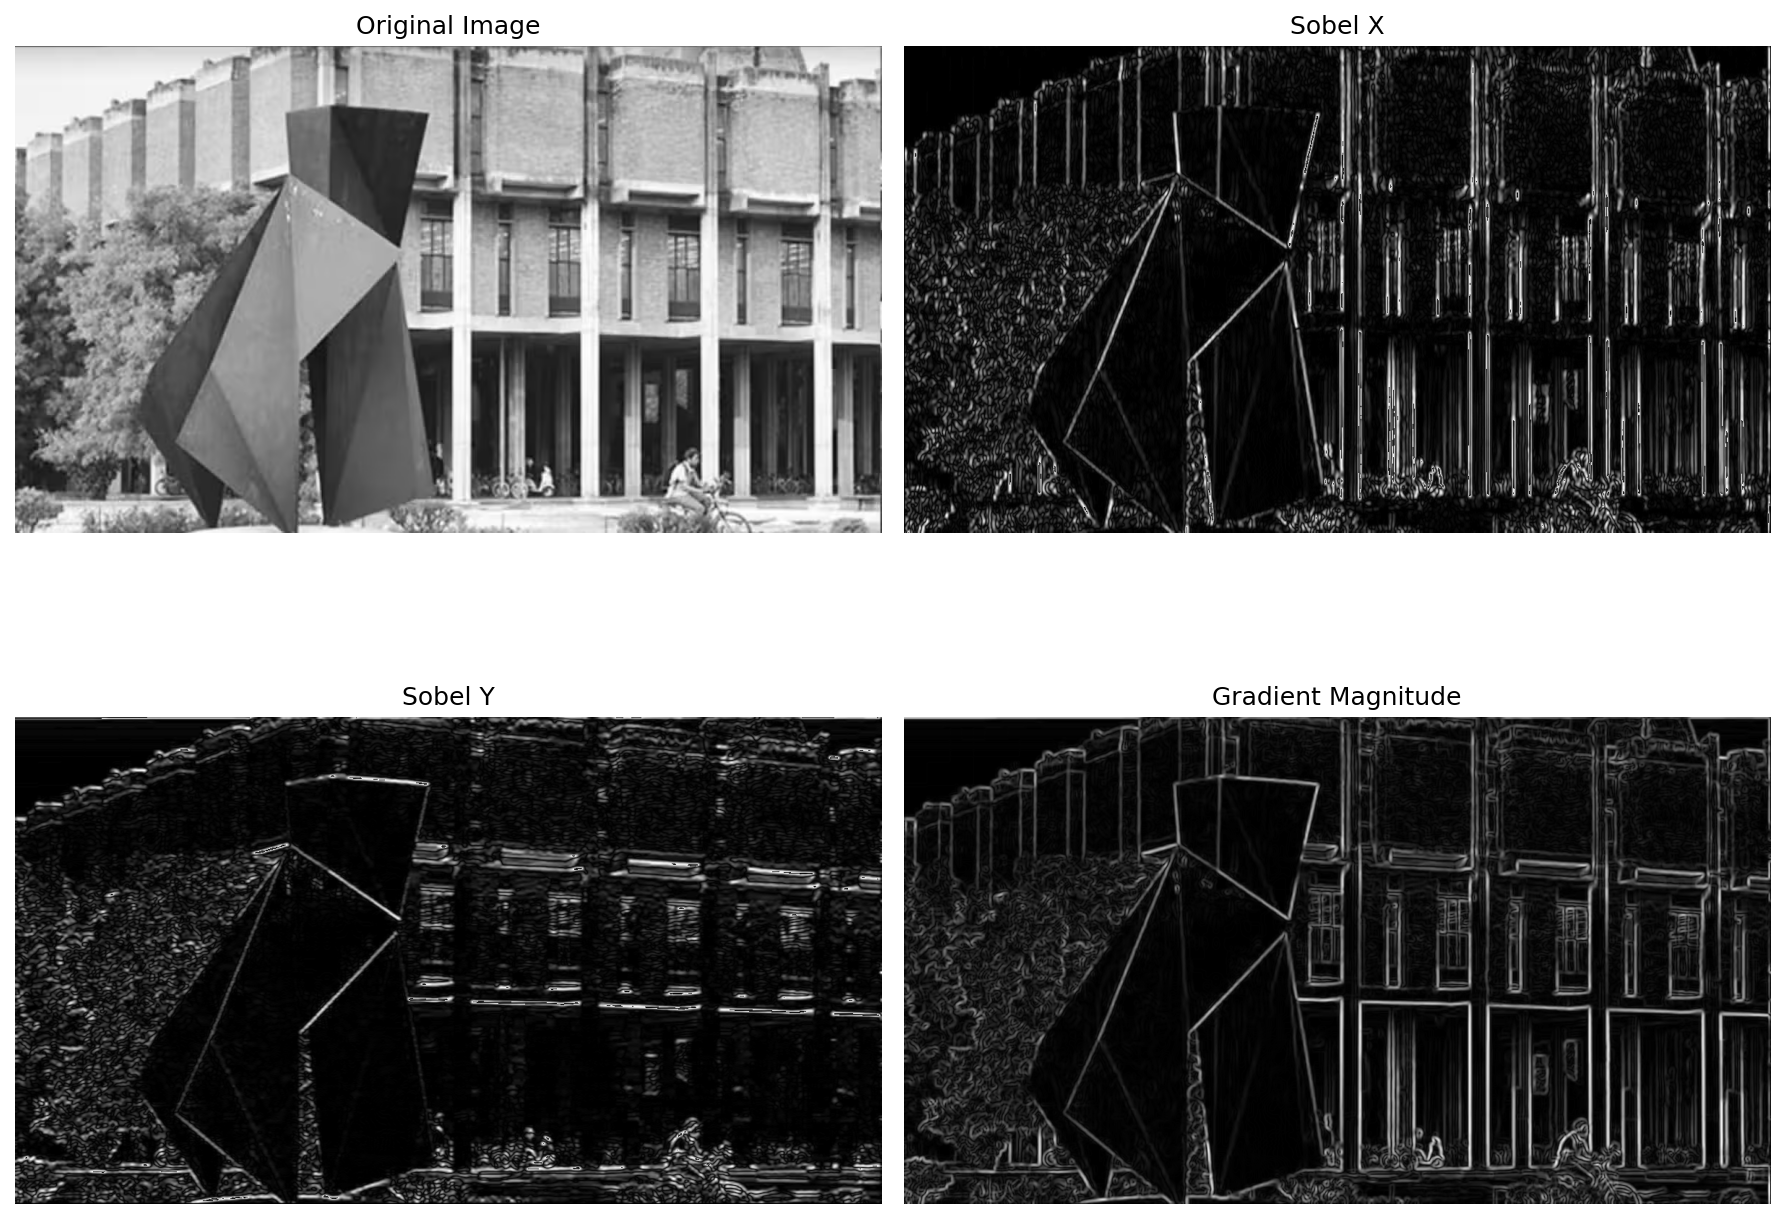
\includegraphics[width=0.85\textwidth]{plots/sobel_smoothed.png}
  \caption{Sobel edge detection results on the Gaussian-smoothed image. From top-left to bottom-right: Original image, horizontal gradient $G_x$, vertical gradient $G_y$, and gradient magnitude. Notice the significant reduction in false edges and noise.}
  \label{fig:sobel_smoothed}
\end{figure*}

Fig. \ref{fig:gradient_comparison} displays a direct comparison of the gradient magnitudes with and without smoothing, while Fig. \ref{fig:difference_map} shows the absolute difference map, illustrating that noise is primarily what is removed by smoothing.

\begin{figure*}[t]
  \centering
  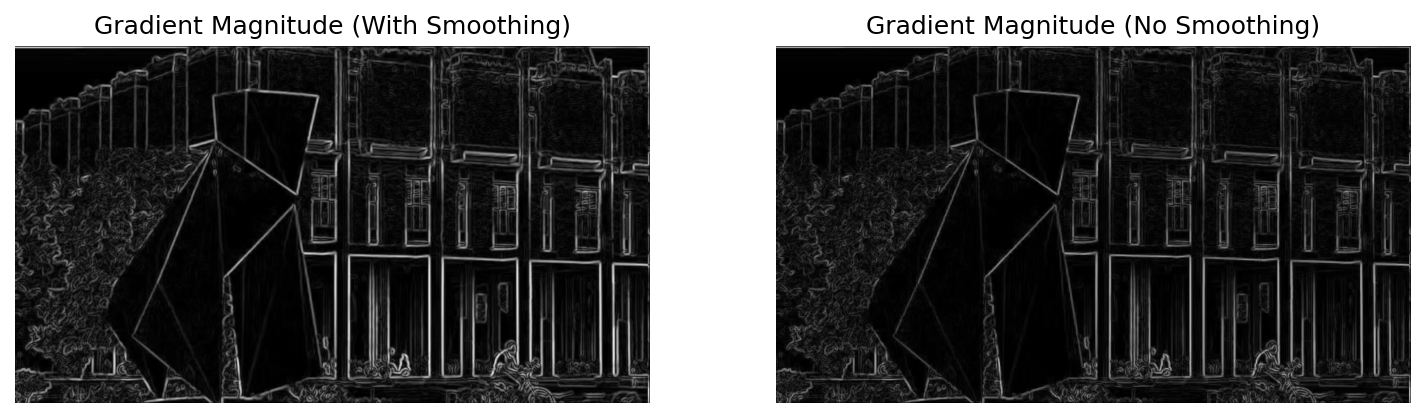
\includegraphics[width=0.85\textwidth]{plots/gradient_comparison.png}
  \caption{Direct comparison between the gradient magnitude obtained with smoothing (left) and without smoothing (right), illustrating how smoothing filters out noisy textures while preserving actual object boundaries.}
  \label{fig:gradient_comparison}
\end{figure*}

\begin{figure}[H]
  \centering
  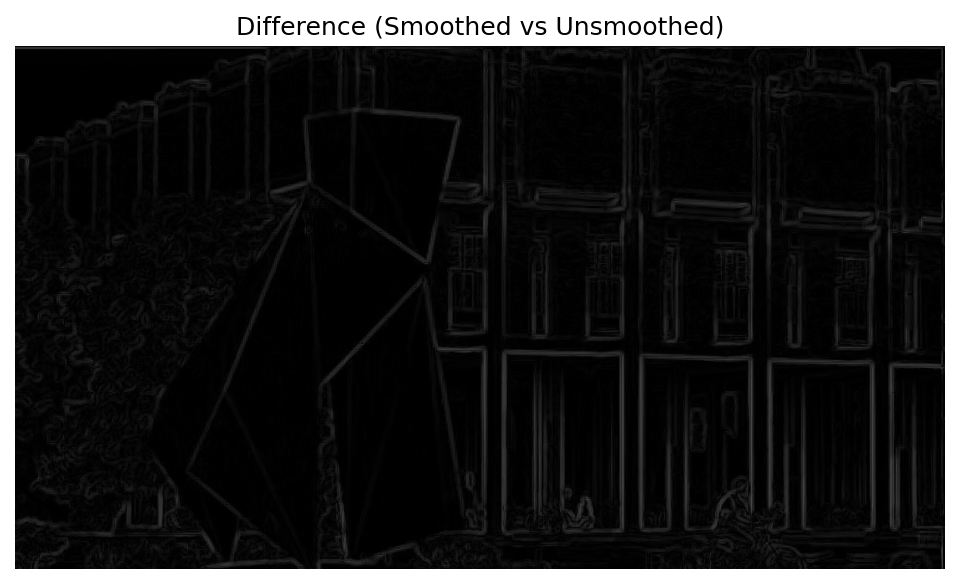
\includegraphics[width=0.85\columnwidth]{plots/difference_map.png}
  \caption{Absolute difference map between the smoothed and unsmoothed gradient magnitudes, highlighting the high-frequency noise that is successfully attenuated by Gaussian smoothing.}
  \label{fig:difference_map}
\end{figure}

Furthermore, thresholding can be applied to obtain binary edge maps. Figure \ref{fig:thresholded_edges} shows the thresholded edge maps at different threshold values: 0.1, 0.2, 0.3, and 0.4. Higher thresholds remove weaker edges and noise, while lower thresholds preserve more fine structural details but may allow noise through.

\begin{figure*}[t]
  \centering
  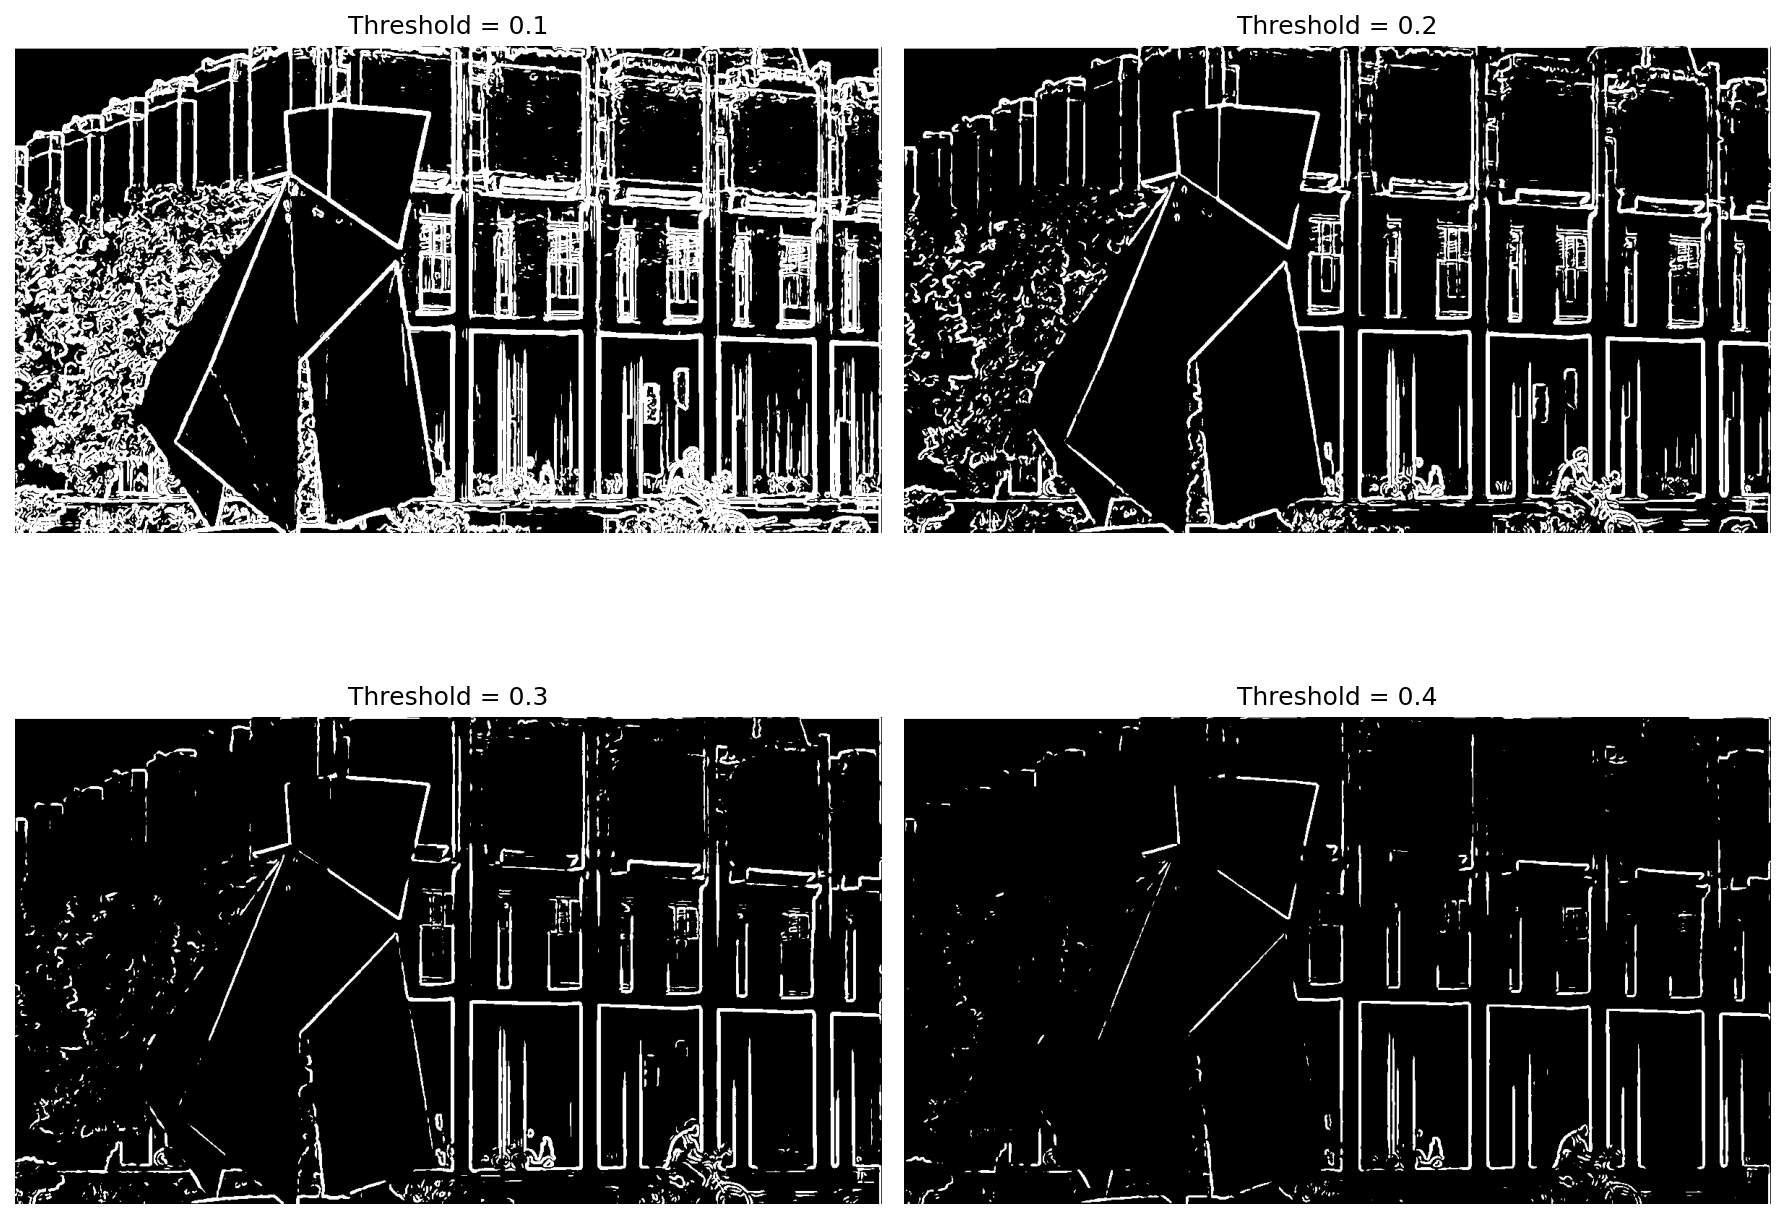
\includegraphics[width=0.85\textwidth]{plots/thresholded_edges.png}
  \caption{Thresholded edge maps at different threshold values: 0.1, 0.2, 0.3, and 0.4. Higher thresholds remove weaker edges and noise, while lower thresholds preserve more fine structural details but may allow noise through.}
  \label{fig:thresholded_edges}
\end{figure*}


% ─────────────────────────────────────────────────────────────────────────────

\section{Discussion}

The results obtained from Q1A demonstrate that periodic interference can be effectively identified and removed in the frequency domain. The selection of notch filter parameters plays a critical role in restoration quality. While larger rejection regions provide stronger noise suppression, they may also remove useful image information and introduce blurring artifacts.

For Q1B, the Sobel operator successfully detected image boundaries through gradient estimation. However, the results also showed that edge detection is highly sensitive to noise. Gaussian smoothing improved edge quality by reducing unwanted high-frequency components before derivative computation.

\section{Applications}

Frequency-domain image restoration techniques are widely used in satellite imaging, surveillance systems, communication receivers and medical imaging to remove periodic interference and sensor artifacts. Similarly, edge detection techniques are fundamental to computer vision applications such as object recognition, autonomous navigation, optical character recognition and image segmentation.

\section{Conclusion}

This work explored two important image processing applications based on concepts from signals and systems. In the first task, Fourier analysis and notch filtering were used to identify and suppress periodic interference, enabling successful recovery of hidden image information. In the second task, the Sobel operator was employed to extract image boundaries, and the benefits of Gaussian smoothing for robust edge detection were demonstrated. The results highlight the effectiveness of both frequency-domain and spatial-domain processing techniques for image analysis and restoration.
% ─────────────────────────────────────────────────────────────────────────────



\end{document}